\chapter{Laços de repeti\c{c}\~ao}

Em Perl quando certa instru\c{c}\~ao precisa ser repetida uma certa quantidade, deve-se fazer uso de um comando de estrutura de repeti\c{c}\~ao, o comando 
\textit{while} \'e um exemplo, \textit{while} significa, ''enquanto''. Vamos usar como base o exemplo na figura 18.

\begin{figure}[!htb]
	\centering
	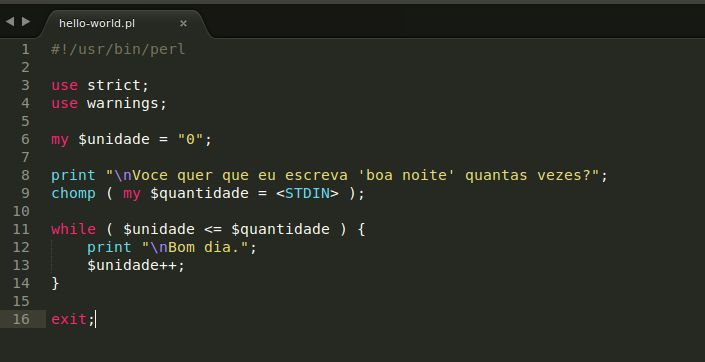
\includegraphics[width=0.5\textwidth]{../5_figuras/image18}
	\caption{Algoritmo com estrutura de repeti\c{c}\~ao while}
\end{figure}

Na 6$^a$ linha definida a vari\'avel \textit{\$unidade = 0}, logo depois, \'e requisitado ao usu\'ario que informe uma quantidade n\'umerica de seu gosto, 
ent\~ao na 11$^a$ linha \'e desenvolvida a seguinte l\'ogica; enquanto \textit{\$unidade $<$= \$quantidade} ser\'a escrito \textit{bom dia} na tela para 
ent\~ao retornar o valor da vari\'avel \$unidade, incrementando-o posteriormente.

\begin{figure}[!htb]
	\centering
	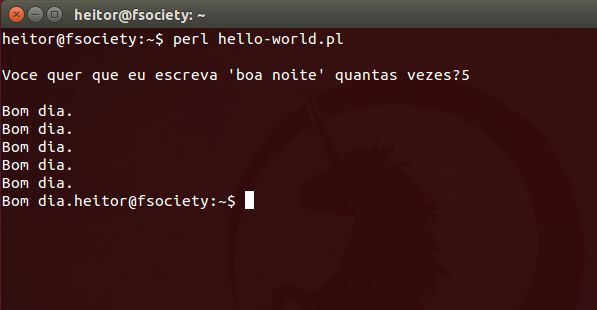
\includegraphics[width=0.5\textwidth]{../5_figuras/image19}
	\caption{Sa\'ida do algoritmo com estrutura de repeti\c{c}\~ao while}
\end{figure}

Outro operador para o mesmo fim \'e o \textit{for}, como \'e apresentado na figura 20.

\begin{figure}[!htb]
	\centering
	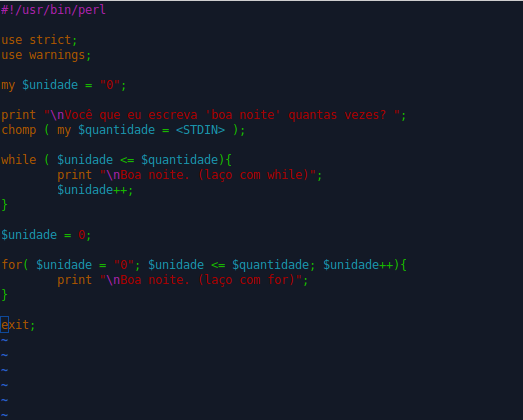
\includegraphics[width=0.5\textwidth]{../5_figuras/image20}
	\caption{Algoritmo com estrutura de repeti\c{c}\~ao for}
\end{figure}

O \textit{while} e o \textit{for} possuem praticamente a mesma finalidade, mas voc\^e deve saber quando usar cada um deles. A sa\'ida desses dois casos 
ser\~ao exatamente iguais.

Que tal deixarmos nossos programas um tanto mais coloridos? Para isso ser\'a usado o m\'odulo \textit{Term::ANSIColor}. Caso sejas um usu\'ario Windows, use 
o m\'odulo \textit{Win32::Console::ANSI}.

H\'a uma grande chance de que sua distribui\c{c}\~ao/SO n\~ao tenha este m\'odulo pr\'e-instalado, para instal\'-lo digite o comando a seguir no terminal 
\textit{cpan install Term::ANSIColor} ou no prompt \textit{cpan install Win32::Console::ANSI} respectivamente. A instala\c{c}\~ao de qualquer modulo segue o 
mesmo padr\~ao, o comando \textit{cpan} chama o mesmo avisando que deve ser instalado o m\'odulo \textit{Term::ANSIColor}. Uma vez conclu\'ida a 
instala\c{c}\~ao, vamos a a\c{c}\~ao!

\begin{figure}[!htb]
	\centering
	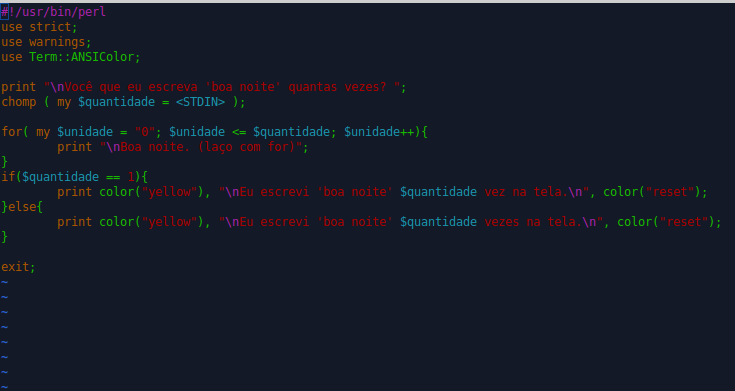
\includegraphics[width=0.5\textwidth]{../5_figuras/image21}
	\caption{Algoritmo com m\'odulo para alterar a cor do texto da sa\'ida padr\~ao do programa}
\end{figure}

Este m\'odulo n\~ao necessita de muita explica\c{c}\~ao, na figura 21, 5$^a$ linha o m\'odulo \'e requisitado e ativado, na sequ\^encia, ocorre uma o envio de
dados para a sa\'ida padr\~ao com a cor que desejes, essa funcionalidade \'e realizada dentro do comando \textit{print}, colocando a cor desejada com a 
seguinte express\~ao \textit{color(''nome'')}. Os nomes das cores devem ser escritos em ingl\^es ingl\^es, ao final do \textit{print} deve-se usar a 
instru\c{c}\~ao de altera\c{c}\~ao das cores com \textit{reset} para retorn\'a-las ao seu estado inicial, como apresentado na figura 22.  

\begin{figure}[!htb]
	\centering
	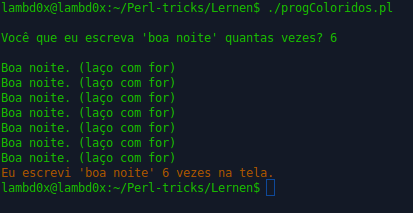
\includegraphics[width=0.4\textwidth]{../5_figuras/image22}
	\caption{Sa\'ida do algoritmo}
\end{figure}

